\begin{titlepage}
\section{Introduction}
Pixel detectors, members of the semiconductor detector family, have fastely been used since the first 
accelerator experiments for energy and position measurement. 
Because of their dimension (today $\sim$ 30 $\mu m$ or even better) and their spatial resolution 
($\sim$ 5-10 $\mu m$), with the availability of technology in 1980s they proved to be perfectly suitable 
for vertex detector in the inner layer of the detector.\\
Hybrid pixel currently constitute the state-of-art for large scale pixel detector but experiments began 
to look at monolitic active pixels (MAPS) as perspective for their future upgrades; some of them, as ALICE or 
(), have already installed them. \\
Hybrid pixels are made by two parts: the sensor and the electronics; for each pixel this two parts are connect 
together through microconnection (bump bond) using the so called flip-chipping tecnology.\\
This particular and sophisticated technique makes hybrid pixels difficult to produce and to test (sensor can't be 
test separatelly but need connection with the readout), delicate, especially for high levels of radiation,
and also expensive. \\
An hot topic for accelerator experiment is the material budget that represents the main limit for momentum measurement
resolution; since MAPS integrate both the sensor and the redout on the same bulk, they are thinner 
($\sim$ 100-150 $\mu m$) than the hybrid ($\sim$ ?? $\mu m$) and they can down the material budget (the typical 
value for hybrid pixels is 1.5 \% $X_0$ per layer) by a third.\\

Among other disadvantages significa più power consumption e quindi anche più cose per raffreddare, che dinuovo
significa aggiunta di altro materiale.\\

Today almost every high energy physics experiment employs semiconductor detector and 
lo sviluppo tecnologico e la ricerca sono indirizzate nel trovare modi per ridurre il material budget e
avere una lettura sempre più veloce: due dei principali limiti attuali per questi detector. \\

Per gli acceleratori la richieste sono molto stringenti soprattutto per il futuro ad es HL LHC in termini di radiation hardness (expected in 5 anni 500 Mrad e NIEL di 10 alla 16), efficiency e occupancy (efficienza alta dopo tanta radiazione e noise occupancy bassa), time resolution (bunch crossing 40 Mhz), material budget e power consumption (material budget below 2per cento e power consumption 500 mW/cm2)

Cos'è la flash therapy\\
Problemi sperimentali della flah therapy\\
Quali sono i limiti sperimentali richiesti per un dosimetro.\\
PERCHè i pixel potrebbero essere buoni per la dosimetria.\\


\begin{comment}
\begin{figure}
    \begin{minipage}{0.48\textwidth}
      \centering
      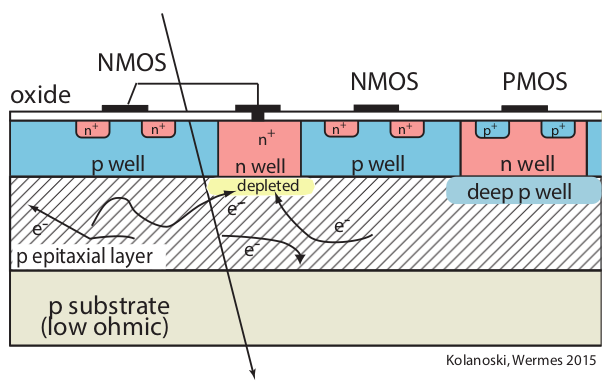
\includegraphics[width=.8\linewidth]{figures/MAPS_scheme.png}
    \end{minipage}
    \begin{minipage}{0.48\textwidth}
      \centering
      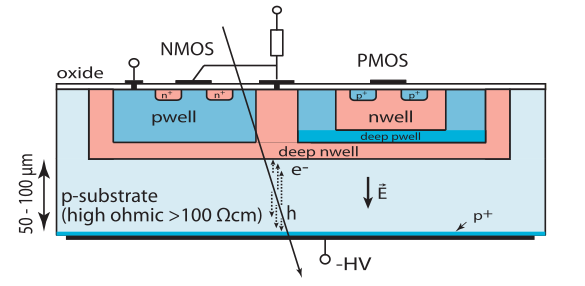
\includegraphics[width=1.\linewidth]{figures/DMAPS_scheme.png}
    \end{minipage}
    \caption{Concept cross section of MAPS and DMAPS pixel}
    \label{fig:MAPS_DMAPS_scheme}
 \end{figure}


 \subsubsection{Position measurement resolution}
Depending on the type of signal reading the spatial resolution is 
$\sigma_x = \frac{p}{\sqrt{12}}$ where $p$ is the pitch between pixels, or even better if other 
analogica information, as the charge, are read and capacitive charge division method is applied.
\end{comment}
\end{titlepage}
